\documentclass{UoYCSproject}

\usepackage{fullpage}
\usepackage{amsmath}
\usepackage{color}
\usepackage{graphicx}

\title{Using Crowd Sourced Information to Understand How Buildings are Used}
\MEng{}
\author{Martin Higgs}
\date{\today}
\supervisor{Iain Bate}
\wordcount{\textcolor{red}{TODO}}

\abstract{
	\textcolor{red}{TODO}
}

\begin{document}
	
	\maketitle
	
	\chapter{Introduction}
    \label{chap:intro}
    
		The aim of this project is to use data from sources such as phones to track where individual people are in building and then this information can be used to learn a model of how the building itself is being used. For instance, models of typical movement patterns, congregation areas etc can be formed. These models can be improved, or cross referenced for verification, with other sources of information, e.g. timetable information, that would suggest who should be in which rooms at what times. The models can then be used for many reasons including optimising the energy usage within a building, e.g. only heat particular rooms shortly before the room(s) is to be used and switch off heating when there is no one in the room(s).
		
		The phases of this project are as follows:
		\begin{enumerate}
			\item Determine and choose from the available sources of information. Where needed augment this with bespoke mobile applications
			\item Investigate how classical machine learning approaches can help derive the necessary models
			\item Derive models from the information obtained
			\item Evaluate the quality of the models using other sources of information
		\end{enumerate}
		The outputs of this project are useful data sets, software for deriving models from the information and a means of evaluating the quality of the models.
		
		The main challenges of this project are:
		\begin{itemize}
			\item Determining which sources of information can easily be used
			\item Deriving means of determining whether a model is good
			\item Producing useful models from unreliable information from a diverse set of sources
			\item Determining credible independent sources of information to compare the information against
		\end{itemize}
        
        \textcolor{red}{Interesting ethical point: I believe most smartphones (Android, iOS and Windows) request to send visible access points back to a central server for mapping availability. By developing this technique could I be inadvertantly mapping every building in the world (private and public alike) with the sheer volume of smartphones available? This is good for things like emergency services, but where do I draw the line?!}
        
        \textcolor{red}{Conclude with a breakdown of what the following sections (chapters at the moment) aim to achieve.}
        
        Estimated length Breakdown (number of words for BSc):
        \begin{itemize}
        	\item Abstract, ethics statement, etc. - 500 \textcolor{red}{(0)}
        	\item Introduction - 1,000 \textcolor{red}{(0)}
        	\item Literature review - 3,000 \textcolor{green}{(4,104)}
        	\item Problem description/analysis - 1,500 \textcolor{red}{(0)}
        	\item Design and implementation - 2,500 \textcolor{yellow}{(800)}
        	\item Results and evaluation - 2,500 \textcolor{red}{(0)}
        	\item Conclusion - 1,000 \textcolor{red}{(0)}
        \end{itemize}
	
	\chapter{Related Work}
    \label{chap:related}
	
		This chapter conducts a review of various works surrounding the project's goals. First it will address the motivations and support the relevance of this study (Section \ref{sec:motivations}). Concluding that it will provide coverage of the constituent parts relevant to the work on crowd-sourcing the data to be used, indoor positioning systems for creating a location map of the data and finally the automated generation of floor plans for analysis of the building in sections \ref{sec:crowd}, \ref{sec:ips} and \ref{sec:floorplans} respectively.
        
        \section{Motivations}
        \label{sec:motivations}
        
            Modelling a building by various methods for automation and analysis can provide a multitude of benefits through better understanding of its use from emergency situation handling to day-to-day improvements. For example \citet{gao2009self} provide an extremely simple method for intelligently setting the on/off times for central heating, increasing energy efficiency while minimising user discomfort. The method is built around using smart-home sensors (such as reed switches on doors or motion detectors) to determine the latest leaving (to work) and earliest entrance (from work) times and incorporating these with a user-specified amount of ``miss time'' when the house is occupied but the house is not already warm. As the technique is solid, with the prevalence of WiFi enabled personal devices, it could easily be adapted to monitor user's devices leaving / moving around the WLAN and scaled to larger buildings with finer grain control over their heating.
            
            By giving the system control over a user's environment however, it enters into a category of ``physical computing systems'' as identified by \citet{stankovic2005opportunities}. While this is a very simple definition of any system that can take in data through some collection of sensors (e.g. a Wireless Sensor Network) and act upon that data through some actuators, one must be aware of the responsibility placed upon the system. Most of the concerns raised are context sensitive, but when designing such a technique it can help to consider these situations in order to identify its limitations. Examples of such systems might include the use of WiFi signal scattering to detect and alert of falls in vulnerable homes \citep{han2014wifall}, provision of city-wide traffic management through a wireless network of cameras and signals \citep{LATraffic} or asset and personnel tracking across a wirelessly networked environment \citep{Ekahau}.
		
            The idea of leveraging wireless networks and the multitude of sensor-enabled devices that occupy them however has been around for quite some time. Recently \citet{torres2014ujiindoorloc} identified the specific trend for using such devices to provide Indoor Positioning / Localisation Systems (IPS), but no definitive way of comparing techniques applied and so created the UJIIndoorLoc database. We will expand upon this data set later, but for now it serves to show the collaborative effort going into solving the problem of indoor localisation.
                
        \section{Crowd-sourcing Data}
        \label{sec:crowd}
        
            With the sheer variety of sensors available in modern personal devices carried by people of all backgrounds almost everywhere, sourcing as much data as possible would seem to be relatively easy. However, when using this technique the data collection must always attempt to be as un-invasive as possible. 
            
            An early endeavour into this field was CenceMe, a classification program designed to relay information about the user to their friends through Facebook \citep{miluzzo2008sensing}. The program ran on the Nokia N95 passively collecting data whenever the phone was interacted with (i.e. through button presses) which were then translated through a simple set of classifications into facts to pass on to the server for processing to Facebook. Collected data included GPS location, microphone noise, accelerometer data, Bluetooth device visibility and random pictures for determining where the user was, whether they were having a conversation, their activity level, who they were with and verification purposes respectively. Initially, the user needed to define people and places significant to them for the classifier to recognise but after this, CenceMe only needed prompt the user for input if it recognised a place the user visited frequently, in order for them to add it as a location to notify their friends about.
            
            Concerns raised during this study included those of privacy, portability, ease of development and power usage, most of which have been addressed by advances in mobile operating systems such as Android and iOS. When developing for the N95 the CenceMe team reported very limiting factors designing their framework including low memory, computational power and general programmability, all of which are not of concern today with multi-core, multi-gigabyte RAM devices running almost complete editions of Java with expansive APIs.
            
            However, with increased capability comes increased potential load on the device's power supply (high-speed cellular internet access and HD video processing are particular culprits), limiting its availability; as such manufacturers, OS providers and researchers alike are continually looking into power saving methods. One such team of researchers looked into a technique they called ``Piggyback Crowd-Sensing'' \citep{lane2013piggyback}. This technique centres around the multi-functional abilities of the devices carried today, for example the GPS sensor may be used for geo-tagging pictures, navigation or social media posts. This provides a crowd-sensing application with a variety of opportunities to utilise the GPS without powering up and winding down the sensor specifically to take measurements; `piggybacking' off of another applications sensor usage. 
            
            The problem with this technique arises with the need to narrow down the window of when / where sensor readings are taken as user application usage can be quite sporadic. The research team then complemented this method with a ``Sensing Decision Engine'' (prediction algorithm) that gathers data on which sensor-using apps were launched in which time windows (6 hour slots of each day), whether it was the weekend or a weekday when it was called up and which square kilometre it was used in. Based on these data, the algorithm is then able to predict whether a sensor is likely to be used in the current situation and so whether it should wait for the sensor to come into use or to power it up on its own. This technique as a whole was shown to save up to 90\% of the energy required to perform crowd-sensing for a small cost to accuracy of readings. Successes in approaches like these have lead to adoptions at an operating system level, such as the Android ``Sensor Batching'' approach \citep{AndroidSenseBatch}.
            
            The location required for this sensing decision engine is intentionally broad as very low accuracy location estimates can be made through triangulation from nearby cellular signal towers. Gathered data however can require a much finer grain location estimate to associate with in order to make it meaningful.
                
        \section{Indoor Positioning Systems (IPS)}
        \label{sec:ips}
        
            Outdoor positioning sensors are commonplace in most devices today with GPS being the dominant technique as a device can calculate its absolute position using only the visible satellites for trilateration. Indoor positioning however often requires a much finer level of precision and with GPS being largely invisible from indoors the problem is widely regarded as being unsolved such to the point that competitions are being regularly held to encourage new techniques \citep{MSLOCComp}. These can be split into  the infrastructured and infrastructureless categories where the former requires deployment of additional equipment around the environment (such as motion sensors or microphones) and the latter should not with the sole exception being the assumed existence of Wireless Access Points (APs).
            
            As a fundamental component of analysing what rooms are in use when is knowing where users are at a given time, this section will cover a variety of IPS techniques in detail. As such each technique will be judged by its pre-deployment effort (cost of extra infrastructure, measurement taking, computational cost etc.), level of prior knowledge required of the building and on-line (active) location accuracy.
            
            \subsection{Early Techniques}
            \label{sec:early}
            
                One of the earliest infrastructured approaches was the Active Badge Location System wherein personnel badges were equipped with infrared emitters sending uniquely identifying signals to be picked up by detectors set up in every room \citep{want1992active}. While the set-up proved extensible (up to 128 badges monitored at once with low conflict rate) and flexible (more sensors can be added / moved with the building) with cheap sensors and badges it still required detectors being wired into every room and as such could only provide room-level accuracy at best and only a vague idea of where each person had been in areas not covered by detectors (such as corridors). 
            
                The team also appears to cite ``radio signals that can penetrate the partitions found in office buildings'' as a negative effect as their technique utilises proximity as a binary indicator of where a person is. However, while the paper may have served as an inspiration to create proximity-based positioning techniques, many more modern methods have decided to use the radios in Wireless APs as a single AP can cover a much larger space than an IR detector. This raises additional challenges though in dealing with how radio signals propagate, as the strength of a radio signal can be mangled by the distance it's travelled,  the materials it's passed through (be it air, wood, jeans or people) and by waves themselves (electromagnetic waves can cause destructive and constructive interference on their own frequency, be they reflected or just transmitted from another source)! Given all of these problems \citet{whitehouse2007practical} evaluated the use of received Radio Signal Strength Indicators (RSSI) as a sole measure to judge distance. Their results confirmed that even in ideal outdoor situations with few obstructions ``small differences in vegetation such as the height of grass can have large effects on RSSI'' and ``Experiments in an indoor environment revealed no discernible pattern in RSSI, even in a large room with no walls and at the very lowest transmission power.''.
            
                Despite this potential for wildly fluctuating RSSI based on the environment \citet{bahl2000radar} were able to create a mathematical model for the RSSI based on the floor plan of the building in question; RADAR, one of the first infrastructureless IPS techniques. RADAR is built around their Wall Attenuation Factor (WAF) model:
            
                \begin{equation} \label{eq:WAF}
                    P(d) = P(d_0) - 10nlog\left(\frac{d}{d_0}\right) - \left\lbrace 
                        \begin{matrix}
                            nW * WAF & nW < C \\
                            C * WAF  & nW \geq C \\
                        \end{matrix}
                    \right.
                \end{equation}
            
                This model is a simple combination of the standard signal path loss model and a linear drop in power for each wall that the signal travels through. To break it down, $P(d)$ is the expected RSSI (in $dBm$) at distance $d$, where $d_0$ is a distance of $0$m or the access point's `Transmit Power'. This signal travelling through the air then decays logarithmically according to an unknown but fixed rate $n$. Finally a fixed amount of power ($WAF$) is lost for each wall ($nW$) up to a pre-determined cap ($C$) beyond which any extra walls make no difference as the signal is pretty much unidentifiable anyway. This model is then applied to approximate the RSSI of every access point at every position in the building (using the floor plan as a guide) the create an RSSI map of the building in question. Location is then a relatively simple task of matching up the user's visible RSSI from each access point and matching them to the closest approximate location. This technique was created to as an alternative to taking `empirical' measurements throughout the building to create the map by hand and while it is not as strong as taking empirical measurements (roughly 30\% increase in median error) it saves a significant amount of effort for such a simple model.
                
                \begin{figure}[h]
                    \label{fig:m2}
                    \caption{Model $M_2$ from \citet{madigan2005bayesian}.}
                    \centering
                        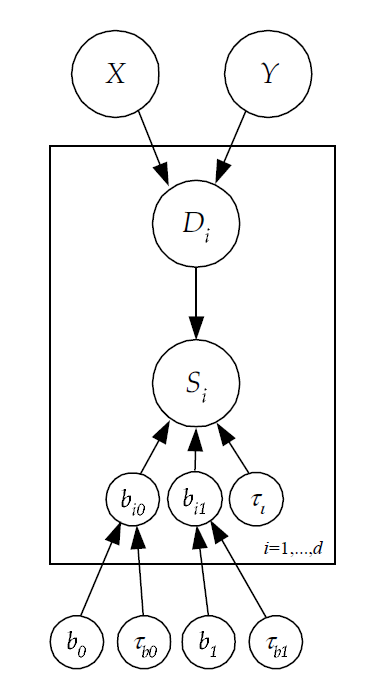
\includegraphics[width=0.3\textwidth]{Model_M2.png}
                \end{figure}
                
                \citet{madigan2005bayesian} instead utilised a graphical model to embody the relationship between position and RSSI (Figure \ref{fig:m2}). In their Bayesian Network, for each access point $i$ the distance $D_i$, transmit power $b_{i0}$, path loss rate $b_{i1}$ and noise $\tau_i$ are all conditionally dependant given the RSSI observed $S_i$. This signifies that given a set of these variables, the model can infer the most likely values for any connected values in the graph (for example, training data would give the X and Y co-ordinates and the signal strength, which can be used to infer all other variables given the graph's complete connected nature). Then during the on-line positioning phase, the user's most likely position is inferred from the AP variables established during the training phase and the observed RSSI values. Using this model they are able to estimate position assuming only the degradation of RSSI is roughly logarithmic and that all access points have similar behaviours ($b_0$ and $b_1$ are the global variables around which each specific access point's values are estimated). This method does require training data in order to calculate the maximum likelihood access point parameters, but with a very small number of training samples (around 20) and no other knowledge of the building they show that the model is able to estimate the user location with a ~50\% increase in median error compared to RADAR.
                
                While providing insights into the area under observation with little prior knowledge, these techniques are 'one-shot': a model is built from known values and then followed permanently thereafter. However, should the space be modified at any point after the model is created, the solution would effectively need re-deploying to continue providing accurate estimates.
            
            \subsection{Adaptive Indoor Positioning Systems}
            \label{sec:adaptive}
            
                All of the previous techniques discussed have had two very distinct phases: off-line and on-line. During the off-line training phase, data is gathered with ground truths (guaranteed values such as user verified location) or models are calculated and then in the on-line positioning phase the observed RSSI values are then used in the models to determine the user's most likely location. This section however will explore techniques that can improve gradually over time as more users traverse the space.
                
                Techniques covered to this point rely on electromagnetic waves and the detection thereof to paint a picture of the user's current location, however \citet{wang2012no} combined dead-reckoning (estimating relative location by tracking movement from a known point) and a broader range of sensors than most other techniques to estimate location. Traditional dead-reckoning is known to be relatively accurate at first, but random errors gradually accumulate and the estimation can become wildly inaccurate the further travelled from the starting point. This technique however relies on organically generated `landmarks' to help reset the accuracy of a user's current position as frequently as possible (Figure \ref{fig:dead}). These landmarks can range from elevators detected by accelerometer spikes to metallic areas detected by the magnetometer, each uniquely identified by the RSSI values surrounding the area. As the mean of the error generated by dead-reckoning is theoretically $0$, a landmark can be placed at the average location of all positions it has been identified at making exact positioning when the landmark is detected possible. While accurate to a reported 1.2m with no prior knowledge of the space and no deployment necessary, this positioning method must be permanently active from each landmark or the user will be unable to locate themselves. Also, even with techniques identified to only use the most effective landmarks this would still put a relatively heavy weight on the user's power supply through its always-on nature and the variety of sensors required compared to conventional RSSI measurement.
                
                \begin{figure}[h]
                    \label{fig:dead}
                    \caption{Dead-reckoning accuracy found through experimentation by \citet{wang2012no}.}
                    \centering
                        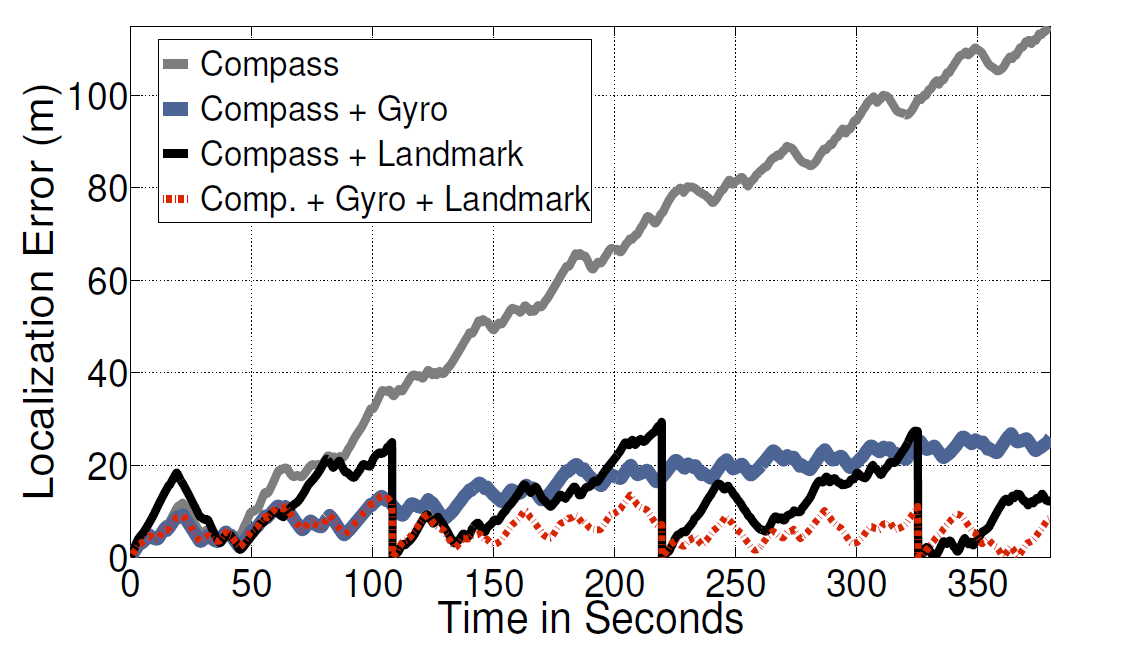
\includegraphics[width=0.7\textwidth]{dead.png}
                \end{figure}
                
                Such conventional methods had also been gradually improved upon to provide sub-metre levels of accuracy using by combining crowd-sourced data with probabilistic reasoning through a technique called `Horus' \citep{youssef2005horus}. The first step (and largest weakness) of the Horus system is the necessary collection of sample data from known locations to create an initial RSSI map. Data collected by users while positioning however now continues to feed back into the initial RSSI map as the team discovered that RSSI values from each AP are not independent with regards to time, so utilise an auto-correlation co-efficient ($\alpha$) to help isolate useful measurements. This co-efficient defines how similar readings in an area have been and augments the expected distribution of RSSI values for that area to allow for a much larger range if all observations have been very similar.
                
                Using this modified RSSI map, positioning is then broken down into multiple steps; first the user's `discrete' area must be determined as the most likely position, given all of the access points that are currently visible. From here, the system uses a function of both the $N$ most likely locations weighted according to their normalised probabilities and the average signal strengths over a small time window to smooth out the estimate. Finally, the system enables tracking of small-scale variations by noting that a user's location cannot change more than their speed would allow. By this notion, if the user appears to have moved more than a threshold amount more than their previous movement, a small-scale error is assumed so the system tries an estimation for all received AP RSSIs multiplied by $1$, $1+d$ and $1-d$ to find the highest likelihood and associated location.
                
                The final technique this paper will cover requiring no prior knowledge of the space, extra deployments or specific training set is Microsoft's `EZ' localisation system \citep{chintalapudi2010indoor}. The technique is centred around solving simultaneous equations to provide accurate estimates, similar to \citet{madigan2005bayesian} in looking for its parameters. However, the technique uses occasional measurements paired with GPS readings and clustering methods to reduce the search space to the most useful subset. 
                
                \begin{equation} \label{eq:EZdistance}
                    d_{ij} = 10^{\left(\frac{P_i - p_{ij}}{10\gamma_i}\right)}
                \end{equation}
                
                For each access point ($i$), the system attempts to solve for its X and Y location, transmit power ($P_i$) and path loss rate ($\gamma_i$). If the access point is visible from at least 5 locations where GPS lock was established ($j$), then these parameters can be uniquely identified through solving simultaneous equations (Equation \ref{eq:EZdistance}) for RSSI values ($p_{ij}$) from which the access point was seen and then using the gathered distances ($d_{ij}$) to trilaterate the 2D location of the AP. Solving even just one AP's parameters can cause a domino effect leading to more uniquely identifiable locations, solving more AP parameters and so on. Eventually though the dominoes stop and the system has to guess some parameters in order to continue and the search space can be incredibly large. To counter this, the EZ team created APSelect and LocSelect, two clustering algorithms that group access points and unknown locations into a single point if the RSSI values observed overlap ~90\%, thereby reducing the number of unknown variables the system has to solve for, taking only a minimal accuracy loss in the process.
                
                The space is then searched through to find a set of parameters with the minimum error using a combination of genetic searching and gradient descent. To start with, a set of solutions with completely random parameters are selected and their fitness (mean absolute error) evaluated. From here, the top 10\% are kept unmodified, 10\% are randomly re-generated, 60\% are made as a combination of 2 random parents from the last generation (and enhancing them through gradient descent) and the last 20\% are made by taking a single random solution from the last generation and tweaking each parameter by a random amount (from an exponential distribution to allow for occasional large changes). This combination of solution generation techniques avoids the large number of potential global minima that come with so many parameters while exploring the state space relatively quickly.
                
                One final optimisation applied to their method is accommodation for relative gain. By identifying proximate locations in which measurements were taken by two different devices, their average RSSI values can be compared to find their approximate relative gain difference and normalise their RSSI values for use in simultaneous equations. With all of these techniques combined, EZ was able to perform comparably to RADAR on larger scale deployments without all of the pre-deployment effort and the search for optimal parameters could be re-run as the space being localised changes and more data comes in. The main disadvantages with this technique come simply from its marginally lower accuracy than techniques like Horus (Figure \ref{fig:EZHorusRADARComparison}) and the relatively high computational effort required to implement the technique and compute the results.
                
                \begin{figure}[h]
                    \label{fig:EZHorusRADARComparison}
                    \caption{Cumulative distribution function of distance error comparing Horus, RADAR and EZ IPS techniques \citep{chintalapudi2010indoor}.}
                    \centering
                        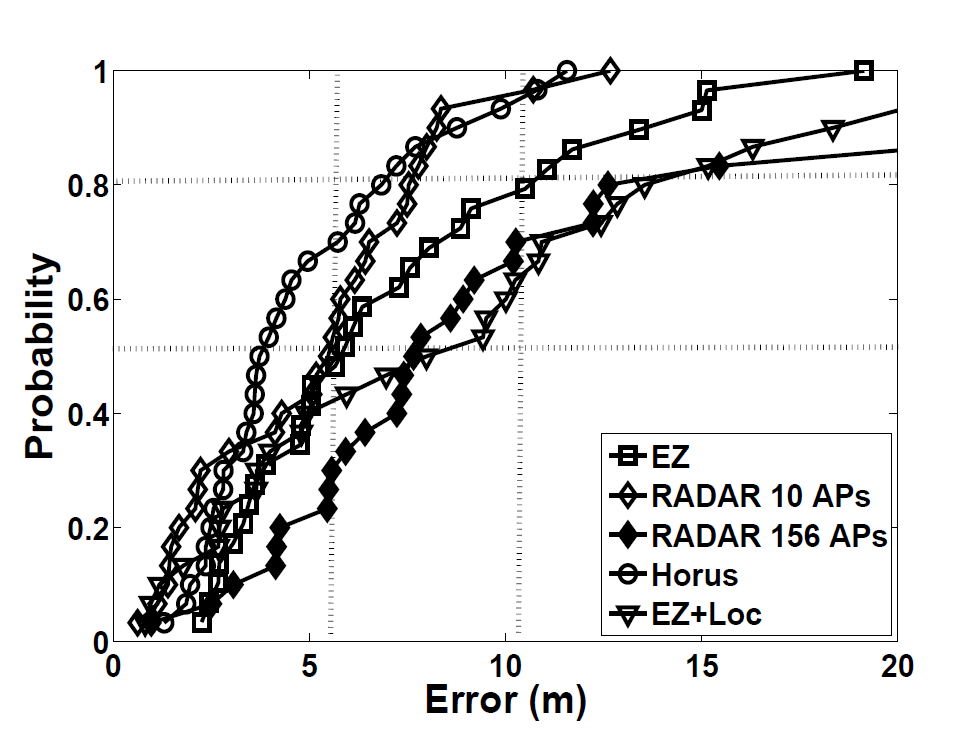
\includegraphics[width=0.7\textwidth]{EZHorusRADARComparison.png}
                \end{figure}
                
                Following the rapid development of IPS techniques \citet{torres2014ujiindoorloc} identified the need for a definitive data set to compare them through and created the UJIIndoorLoc database. The data set comprises of a large number of user-verified co-ordinates and their respective RSSI values to every WLAN access point being monitored. As these measurements were carried out by a number of users (integrating height as a differentiating factor) with a number of devices this provides great ecological validity to the data set while still delivering reliable measurements. The validation set was also generated without guide markers, ensuring that data different from the training set was provided. With such a comprehensive data set it is then easy to emulate limiting factors of any data gathering technique, such as noise or poor coverage, and due to high demand the team also provided a map of the locations \citep{UJIIndoorLocMap}. However, data points extraneous to the buildings in question would have been useful to provide a complete picture of a user's day both inside and outside of the buildings.
            
        \section{Automated Floor Plans}
        \label{sec:floorplans}
        
            Floor plans of a building are often key to enabling detailed location-based analysis by providing boundary information and special characteristics of the space, but may not be available prior to a system's deployment. It is easy to see how a special purpose robot might use a combination of dead-reckoning and obstacle sensors to map a space using an exhaustive search, but the cost of the equipment and the size of the area being surveyed could easily render the technique infeasible.
            
            Other techniques for building floor plans rely on gathering a small amount of pre-requisite data and building upon the constraints that it gives. A technique for determining layout on a small (single floor house) scale is described by \citet{lu2012smart} for use on ``Smart Homes''. Smart homes are buildings with a notion towards autonomous control, such as turning on the lights in the hallway before the user physically enters the space, detected through a collection of sensors placed about the home. Here, it is required to have motion detectors placed on both sides of every door (to determine room connectedness), a magnetometer (to determine door orientation) attached to these pairs of motion detectors and light level sensors on every window (facing inside and out, to determine orientation through sunrise / sunset). While this is a very high deployment cost through the level of user involvement, the deployed sensors are then anticipated to be in continuous use as part of the smart home itself.
            
            By monitoring the sensors to see which sets fire simultaneously, they can then be clustered into rooms to determine how many doors and windows each room has, and which rooms they are connected to. With the room's interconnectedness established, the technique then minimises the space of potential arrangements using a set of simple heuristics (i.e. windows tend to be on external walls and buildings have as few corners as possible). Despite all of these restrictions, the technique was only able to minimise the set to 2 or 3 potential layouts from which a user must select. As this technique was designed to prevent having a user draw their own plan it satisfies its purpose, but does not provide a detailed enough picture for fine-grain analysis or larger areas of observation.
            
            A more general approach to generating floor plans based on a set of constraints however comes from \citet{charman1994constraint}. This method mathematically defines a set of rooms based on their rotation, reference point and dimensions and attempts to fit them into a given space by connecting their corners. As the rooms are placed, a set of constraints are then evaluated and back-tracked upon where necessary (e.g. Bedroom \#1 must be to the right of Bathroom \#2). By exhaustively generating solutions, the system is able to find all possible layouts of rooms, given the pieces of data / constraints supplied. While successful at producing floor plans for traditional housing layouts, the method could fall short with modern architecture that often contains complex shapes (not squares) and unidentified empty spaces.
            
        \section{Conclusions}
        
	        This chapter has now broken down the work surrounding building analysis into the data gathering, data localisation and floor plan generation steps and provided a variety of techniques that are applicable at each stage. When gathering data from users it has been shown that techniques exist to reduce the load placed on users and their devices, potentially increasing the amount of data that would be gathered in a crowd-sourced technique through more opted-in users. While users are of the utmost importance when performing any crowd-based operations, this report focuses mainly on applications of the data once collected.
            
            When localising gathered data, a theme has emerged centring around the use of RSSI to estimate distances from access points. Despite its complex nature, the  widespread use and coverage of wireless networks combined with the success of simple models make it an attractive choice for IPS. Techniques explored here covered the fundamentals of modelling radio signal propagation, then demonstrated more advanced and novel techniques inferring unknown parameters through machine learning for ease of deployment and increased accuracy alike.
            
            Finally sets of constraints were identified for generating possible floor plans based on estimated dimensions. While restrictive in their application to walls in the four cardinal directions, this fits common traditional layouts of buildings and it is anticipated that more complex arrangements could be broken down into rectangular subspaces to build in. Through combinations of the described techniques this report will now explore ways in which a system might determine room usage from a set of simple crowd-sourced data.
            
    \chapter{\textcolor{red}{Problem Analysis?}}

	\chapter{Method}
    \label{chap:method}
	
		This chapter will cover the development of an indoor positioning system from which positioning data and Wireless AP models can be extracted for use as part of a general building model. The  model will follow the techniques as specified in the EZ localisation system \citep{chintalapudi2010indoor} with measurements from the UJIIndoorLoc data set for testing and evaluation purposes \citep{torres2014ujiindoorloc}. This chapter will also identify weaknesses in the specification of EZ and propose the Simplified-EZ localisation system to compensate.
		
		\section{System Specification}
		
            As explored in chapter \ref{chap:related}, there exist a multitude of techniques for localising users in an indoor space with varying degrees of accuracy. The goals of this project however, limit the range of applicable techniques as the model should be created from readily available sources of information. While this immediately rules out any infrastructured techniques as the installation of extra equipment severely limits the domain space that can be modelled, this project will also avoid those that require a large set of ground-truth, domain-wide test data as they are again limited in their application.With these restrictions in place the most interesting systems to study would be: RADAR \citep{bahl2000radar}, landmarked dead-reckoning \citep{wang2012no} and EZ \citep{chintalapudi2010indoor} from those evaluated in chapter \ref{chap:related}.
            
            RADAR provides one of the highest levels of accuracy of all reviewed techniques for relatively low localisation and model-building cost all based around a single source of information: a pre-existing floor plan. In situations where detailed floor plans are already available, using this method could be the most efficient means for determining building usage metrics as the model building process is skipped entirely and user positions can be determined immediately. However, floor plans are not always complete, universally accessible nor consistent with flexible spaces such as exhibition centres. Because of this limitation in combination with the lack of information generated by skipping the modelling process, this technique is not useful for the project.
            
            Landmarked dead-reckoning appears to rectify most of these concerns as the technique requires no previous knowledge of the space and creates its map of landmarks that are potentially much less dependent on the flexible properties of the space (such as elevators and stairs). This enables the modelled space to change over time while preserving a relatively high level of relative location accuracy. Therein however lies the problem with using this technique to measure space utilisation as it can only detect relative movement as opposed to independent single-point localisation. This is not to say that the technique would be difficult to gather sample data as \citet{torres2015ujiindoorlocmag} provides the full complement of magnetometer, accelerometer and (in conjunction with \textcolor{red}{PRIVATE CORRESPONDENCE SAYS RSSI DATA FOR AREA IN COMING}) RSSI readings necessary to implement such a system. The worry is more about the load placed on prospective user's devices and how to gather meaningful results without the storage requirements becoming infeasible. As shown in the UJIIndoorLoc-Mag database, the ~40,000 data points only correspond to ~300 short relative motion traces so it is not unimaginable for the data sets to quickly get out of hand, especially if a user were to store multiple day's worth of data before a storage opportunity arises. Solutions to these problems could involve modifying the sampling frequency to reduce the load on the user's device and the amount of data held for analysis, but it is unknown as to how this would affect the accuracy of the model due to the precise nature of the landmarks. Also, the test data and initial research do not cover the prospect of spending a large period of time walking around the same space with no significant landmarks. In these cases, the behaviour would return to basic dead-reckoning and continually stack up inaccuracies, potentially invalidating the data. For these issues in combination, landmarked dead-reckoning does not significantly work in the project's favour.
            
            EZ however, implements a system requiring a very simple set of independent client-side measurements backed up by a server-side model that can adapt to a changing space as the set of observations grows, without human intervention (such as specifying a new floor-plan like RADAR). 
            
            \textcolor{blue}{Developing this system using samples from a large data set such as the one created by \citet{torres2014ujiindoorloc} will also enable the component to exist independently, with the crowd-sourcing and floor plan modelling strategies being interchanged at will.}
            
            Points covered (2.5 pages):
			\begin{itemize}
				\item Extract requirements from EZ spec and why EZ (4)
				\item Design set of components in UML (pipe \& filter?) and why components (2)
                \item Introduce and justify implementation in Matlab (1)
				\item Test according to claims in paper (compare to large test set) (2)
                \item Explain why only IPS specification here? (1)
				\item \textcolor{red}{Repeat per component}
			\end{itemize}
		
		\section{Data Preparation}
		
			\begin{itemize}
				\item Why data prep first (RGEA run first to reduce artificial noise applied to RSSI measurements at each location). Data localised to much smaller area to prevent invalid scaling (initial readings in meters from lat, long: 0,0) (1)
				\item First version of implementation incorrect (2)
				\begin{itemize}
					\item EZ spec, compare all APs, led to far too many proximate measurements and completely connected graph of relative gains (unsatisfiable)
					\item Mention special modifications to fit with UJIIndoorLoc data set
					\item Using simulated annealing to factor in random element
					\item nchoosek to extract pairs of devices (relative gain is symmetrical)
				\end{itemize}
				\item Implementation of ground truth RGEA for evaluation (noticable speed difference because only comparing the 3 parameters) (1)
				\item Fix RGEA according to faults discovered found through experimentation (2)
				\begin{itemize}
					\item Check for average absolute difference but then gain is average normal difference (think diagram)
					\item Even with restrictions on APs tends to find 1 falsely proximate point, threshold so there is at least a significant overlap (sum(prox) > 10)
					\item Change to system of linear equations, underspecified for number of gains to be solved, but simulated annealing performs far worse (and modifies irrelevant parameters)
					\item Relative gains prioritised by \texttt{sigma\_deltaG}, but this causes exponential increase in priority for very little increase in probability through bell curve.
				\end{itemize}
				\item Simplified RGEA compares only those where the strongest RSSIs were of the same APs. Massive speed gains as only comparing similar number of parameters to ground truth (also sparse). (2)
			\end{itemize}
		
		\section{Heirarchical Clustering}
		
			\begin{itemize}
				\item Emphasize necessity specifically with UJIIndoorLoc as measurements with lots of different devices taken at the same location and EZ requires readings at different distances to prevent skew when performing the GA.
				\item EZ implementation requires \emph{HUGE} amounts of comparisons because of its fundamentally simple nature (profiling shows > 10,000,000 * 520 comparisons for AP clustering alone!)
				\item Renders LocSelect computationally intractible using the UJIIndoorLoc data set
				\item Worth a brief investigation into set clustering techniques? (already pruning on equivalent set discovery)
                \item Try implementing for raw speed in C called from Matlab?
				\item Simplified version using similar techniques to simplified RGEA to speed the process along
			\end{itemize}
		
		\section{Model Creation}
		
			\begin{itemize}
				\item Simulated annealing rather than GA on AP-by-AP basis (assuming independence) for speed of implementation
				\item No real AP parameters specified as part of UJIIndoorLoc, localising data from 2D subspace with 3D readings doesn't work! Confirmed plans to provide more detailed data set in the near future (both the library piece on the website and a set from just their labs). Will test if released in time. (Continue using entire data set for RGEA as should provide most average picture, but then modelling 2D subspaces as techniques are most tested in 2D realm)
				\item Mention possibility of localising in 3D, but increases number of parameters and required equations to solve for respectively
				\item Thresholding idea to split 3D into set of 2D subspaces (does eliminate edge-case measurements which are niche, but powerful in isolating a very particular area of the building such as directly below and AP on the next floor or in the nearest building)
				\item Thresholding parameters (number of max strenght measurements / threshold leve) could be determined through GA again, but this would run the risk of overfitting. State intent to experiment with parameters as they also affect the amount of data that can be localised in the test set.
				\item \textcolor{red}{IMPLEMENT ERSGA}
                \item \textcolor{green}{Demonstrate localisation after model generation (Use RSSI to calculate approximate distance, then solve simultaneous equations for distance to AP)}
				\item Show maturity through completeness and preparation for future use
				\item Simplified model uses only strongest measurements for model creation and localisation; avoids conflicting measurements, increases speed
                \item Comparison with Horus methodology?
			\end{itemize}
        
	\chapter{Evaluation}
    \label{chap:eval}
	
		\textcolor{red}{Save actual quantifiable results for this section! Evaluate against requirements / massive discrepancies in method.}
		\begin{itemize}
			\item Parameter experimentation
			\item Use PlotFloor to show difference between models with various pieces of the system included / excluded and parameters tweaked
			\item Evaluate with noisy and partially localised data
			\item Show validation as well as evaluation of new model - explain increasing threshold will remove potentially useful boundary cases, but remove a large amount of useless noisy data.
			\item Validation should mainly be shown through qualitative justification and explanation, but can be done over a large number of tests (multiple runs on multiple floors and buildings) in the absence of mathematical proof.
			\item Test same parameters across other data sets (library and computer lab) for consistent levels of accuracy
		\end{itemize}
		
		\textcolor{blue}{\emph{\[GOOD PIECES WITHIN\]}Testing should show validation as well as evaluation of the new model. Validation could explain how increasing threshold level will remove APs from other floors, but also potentially remove small overlaps from nearby buildings (i.e. if an AP is visible only in a small area near the edge of the building, seeing that AP means the location must me in that space). A similar effect could potentially be observed across floors (i.e. the AP only being visible if the location is directly below it), but this would require a much wider domain for parameters, such as extremely low transmission powers or extremely high path loss rates. However, use of these extremes, could be identified and used to help place the AP on another floor with some defined loss across floors like the WAF used in RADAR.}
	
	\chapter{Further Work}
    \label{chap:further}
	
	\chapter{Conclusion}
    \label{chap:conclusion}
    
    \textcolor{red}{\emph{MAKE SURE YOU CHECK YOUR REFERENCES ARE CORRECT!}}
        
    \bibliography{report.bib}
	
\end{document}
